\documentclass[12pt]{article}
\usepackage{amssymb,mathtools, systeme}
\usepackage[margin=1in]{geometry}
\usepackage{fancyhdr}
\usepackage{circuitikz}
\usepackage{graphicx}
\graphicspath{ {./Figures/} }
\usepackage{amsmath}
\usepackage{ragged2e}
\usepackage{subcaption} 
\usepackage{float}
\usepackage{cancel}
\usepackage{siunitx}
\pagestyle{fancy}
\usepackage[shortlabels]{enumitem}
\usepackage{mathtools}
\newcommand*{\permcomb}[4][0mu]{{{}^{#3}\mkern#1#2_{#4}}}
\newcommand*{\Comb}[2]{{}^{#1}C_{#2}}%
\DeclarePairedDelimiter\ceil{\lceil}{\rceil}
\DeclarePairedDelimiter\floor{\lfloor}{\rfloor}
\setlength{\headheight}{15 pt}
\lhead{Georgy Antonov}
\chead{HW 6}
\rhead{Neural Dynamics}

\begin{document}\noindent


\noindent\textbf{Question 1. Linear Dynamical System.}
\begin{enumerate}
\item[]We have the following linear dynamical system 
\[
    \dot{\mathbf{x}}(t) = \mathbf{Ax}(t) + \mathbf{s}(t)
\]
where
$$\mathbf{A} = \begin{pmatrix}
    -0.5 & -0.5 & 0\\
    -0.5 & -0.5 & 0\\
        0 &    0 & 2
\end{pmatrix}$$
\item[1.1] Assuming $\mathbf{s}(t)=0$, we need to compute and sketch the solutions for the initial conditions
\[
    \mathbf{x}_{0,1} = \begin{pmatrix} 1\\ 1\\ 0 \end{pmatrix}, \quad 
    \mathbf{x}_{0,2} = \begin{pmatrix} 1\\ 0\\ 0 \end{pmatrix}, \quad
    \mathbf{x}_{0,3} = \begin{pmatrix} 0\\ 1\\ 0 \end{pmatrix}, \quad
    \mathbf{x}_{0,4} = \begin{pmatrix} 0\\ 0\\ 10^{-6} \end{pmatrix}
\]

Note that the initial value problem has a solution of the form
\[
    \mathbf{x}(t) = e^{\mathbf{A}t} \mathbf{x}_{0}
\]
For non-singular $\mathbf{A}$, we can rewrite it as follows
$$\mathbf{x}(t)=\mathbf{Q}e^{\mathbf{\Lambda} t}\mathbf{Q}^{-1}\mathbf{x}_{0}$$
where $\mathbf{Q}$ is a matrix of eigenvectors and $\mathbf \Lambda$ is a daigonal matrix with non-zero entries representing corresponding eigenvalues.
To solve this, we have to first find the eigenvalues and eigenvectors of $\mathbf{A}$. 
Hence, we start by solving the characteristic equation
\[
    \text{det}\left(\mathbf{A} - \mathbf{I}\lambda\right) = 0
\]
\[
\begin{vmatrix} -0.5 - \lambda & -0.5 & 0\\ -0.5 & -0.5 - \lambda & 0\\ 0 & 0 & 2-\lambda \end{vmatrix}
    = 0 \quad \iff \quad -\lambda^{3} + \lambda^{2} + 2\lambda = 0
\]
We find that $\mathbf{A}$ has three distinct eigenvalues, namely, $\lambda_{1}=0, \, \lambda_{2}=2, \, \lambda_{3}=-1$, with 
the corresponding eigenvectors
\[
\mathbf{v}_{1}=\begin{pmatrix} -1\\ 1\\ 0 \end{pmatrix}, \quad \mathbf{v}_{2}=\begin{pmatrix} 0\\ 0\\ 1 \end{pmatrix}, \quad \mathbf{v}_{3}=\begin{pmatrix} 1\\ 1\\ 0 \end{pmatrix}
\]
Now, we have
\begin{align*}
    \mathbf{Q}=\begin{pmatrix} -1 & 0 & 1\\ 1 & 0 & 1\\ 0 & 1 & 0 \end{pmatrix}, & \quad \mathbf{\Lambda} = \begin{pmatrix} 0 & 0 & 0\\ 0 & 2 & 0\\ 0 & 0 & -1 \end{pmatrix}
\end{align*}
and we can thus write our solution as follows
\begin{align*}
\mathbf{x}(t) &= \begin{pmatrix} -1 & 0 & 1\\ 1 & 0 & 1\\ 0 & 1 & 0 \end{pmatrix}
                \begin{pmatrix} 1 & 0 & 0\\ 0 & e^{2t} & 0\\ 0 & 0 & e^{-t} \end{pmatrix}
                \begin{pmatrix} -1 & 0 & 1\\ 1 & 0 & 1\\ 0 & 1 & 0\\ \end{pmatrix}^{\!-1}\mathbf{x}_{0}\\
\implies \mathbf{x}(t) &= \begin{pmatrix} -1 & 0 & 1\\ 1 & 0 & 1\\ 0 & 1 & 0 \end{pmatrix} \begin{pmatrix} -0.5 & 0.5 & 0\\ 0 & 0 & e^{2t}\\ 0.5e^{-t} & 0 & 0\\ \end{pmatrix}\mathbf{x}_{0}\\
\implies \mathbf{x}(t) &= \begin{pmatrix} 0.5+0.5e^{-t} & -0.5 & 0\\ -0.5+0.5e^{-t} & 0.5 & 0\\ 0 & 0 & e^{2t}\end{pmatrix}\mathbf{x}_{0}
\end{align*}
And in a non-matrix form this becomes 
\[
\mathbf{x}(t)=\begin{pmatrix} (0.5 + 0.5e^{-t})x_{1} - 0.5x_{2}\\ (-0.5 + 0.5e^{-t})x_{1} + 0.5x_{2}\\ e^{2t}x_{3}\end{pmatrix}
\]
Finally, for the aforementioned initial conditions, we have
\begin{align*}
\mathbf{x}_{0,1}(t)&=\begin{pmatrix} 0.5+0.5e^{-t} & -0.5 & 0\\ -0.5+0.5e^{-t} & 0.5 & 0\\ 0 & 0 & e^{2t}\end{pmatrix} \begin{pmatrix} 1\\ 1\\ 0 \end{pmatrix} = \begin{pmatrix} 0.5e^{-t}\\ 0.5e^{-t}\\ 0 \end{pmatrix}\\
\mathbf{x}_{0,2}(t)&=\begin{pmatrix} 0.5+0.5e^{-t} & -0.5 & 0\\ -0.5+0.5e^{-t} & 0.5 & 0\\ 0 & 0 & e^{2t}\end{pmatrix} \begin{pmatrix} 1\\ 0\\ 0 \end{pmatrix} = \begin{pmatrix} 0.5+0.5e^{-t}\\ -0.5+0.5e^{-t}\\ 0 \end{pmatrix}\\
\mathbf{x}_{0,3}(t)&=\begin{pmatrix} 0.5+0.5e^{-t} & -0.5 & 0\\ -0.5+0.5e^{-t} & 0.5 & 0\\ 0 & 0 & e^{2t}\end{pmatrix} \begin{pmatrix} 0\\ 1\\ 0 \end{pmatrix} = \begin{pmatrix} -0.5\\ 0.5\\ 0 \end{pmatrix}\\
\mathbf{x}_{0,4}(t)&=\begin{pmatrix} 0.5+0.5e^{-t} & -0.5 & 0\\ -0.5+0.5e^{-t} & 0.5 & 0\\ 0 & 0 & e^{2t}\end{pmatrix} \begin{pmatrix} 0\\ 0\\ 10^{-6} \end{pmatrix} = \begin{pmatrix} 0\\ 0\\ 10^{-6}e^{t} \end{pmatrix}
\end{align*}
And the phase diagrams for these initial conditions appear in Figures 1-4.
\begin{figure}[h!]
    \centering
    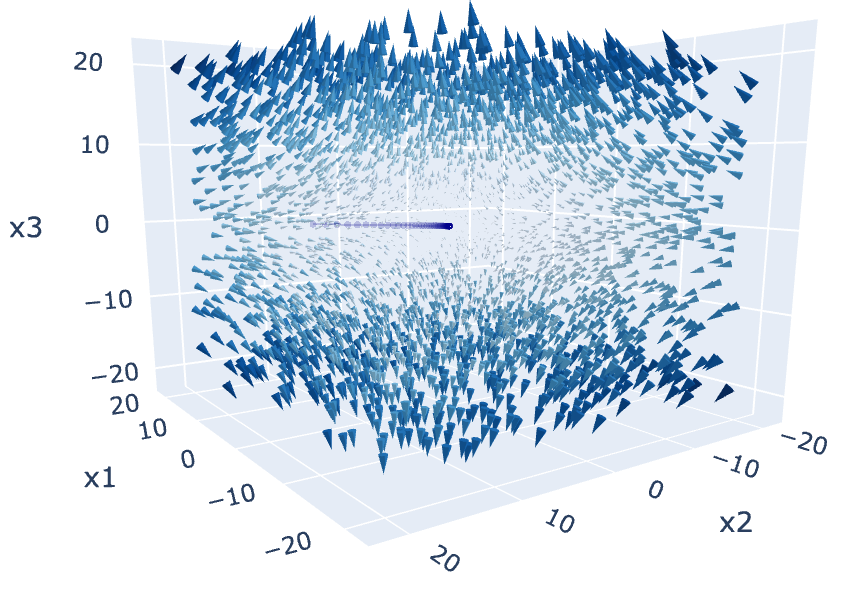
\includegraphics[width=1\textwidth]{Figures/1.png}
    \caption{3D dynamics of $\mathbf{x}(t)$ following the initial condition $\mathbf{x}_{0,1}$ for $t \in [-3, 3]$.}
\end{figure}
\begin{figure}[h]
    \centering
    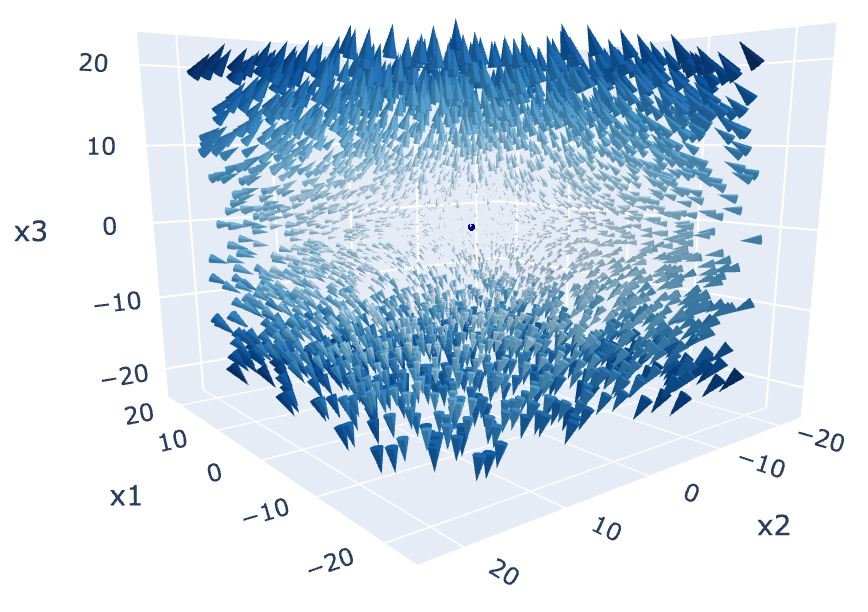
\includegraphics[width=1\textwidth]{Figures/2.png}
    \caption{3D dynamics of $\mathbf{x}(t)$ following the initial condition $\mathbf{x}_{0,2}$.}
\end{figure}
\begin{figure}[h]
    \centering
    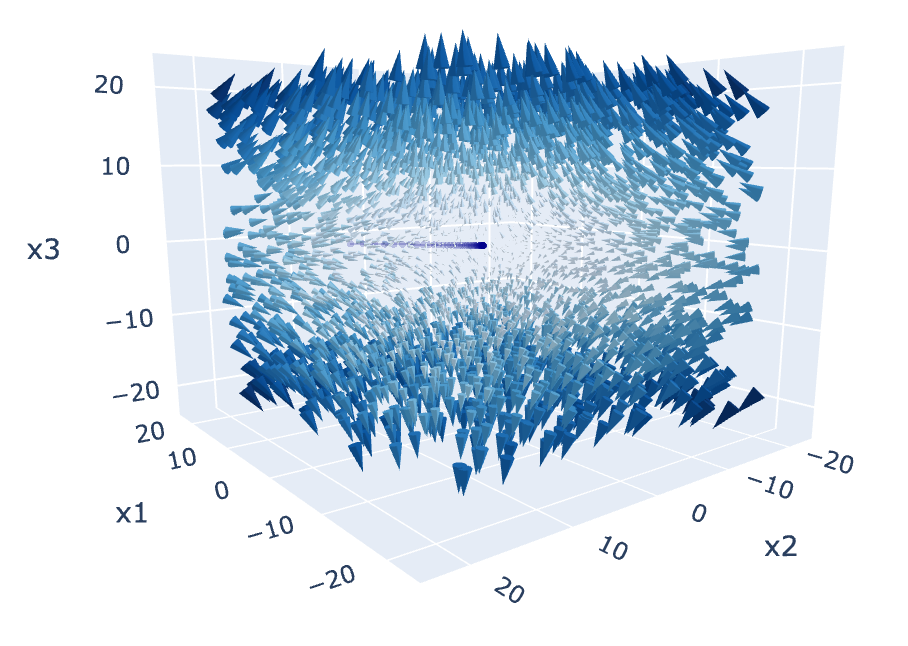
\includegraphics[width=1\textwidth]{Figures/3.png}
    \caption{3D dynamics of $\mathbf{x}(t)$ following the initial condition $\mathbf{x}_{0,3}$ for $t \in [-3, 3]$.}
\end{figure}
\begin{figure}[h]
    \centering
    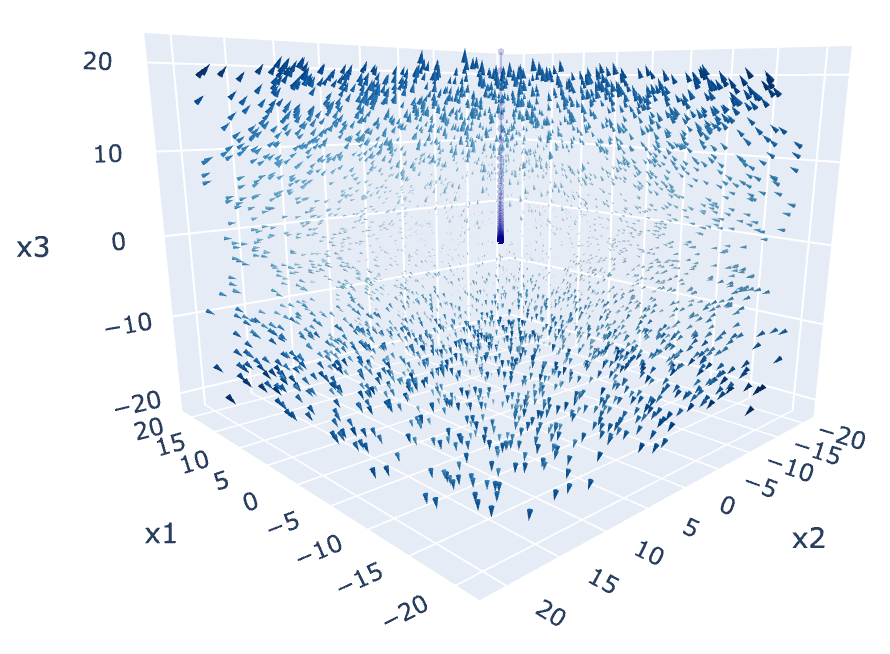
\includegraphics[width=1\textwidth]{Figures/4.png}
    \caption{3D dynamics of $\mathbf{x}(t)$ following the initial condition $\mathbf{x}_{0,4}$ for $t \in [-17, 17]$.}
\end{figure}
\item[1.2] The eigenvalues and eigenvectors of $\mathbf{A}$ were computed in 1.1. Eigenvalue sign tells us about
the direction and speed of the dynamics evolution, and the eigenvectors tell us in which direction the flow will be linear, i.e. only 
affected by the dynamics matrix as a scalar multiplication. 
\item[1.3] The projections of $\mathbf{f}(\mathbf{x})=\mathbf{Ax}$ appear in Figures 5-7.
\begin{figure}[h]
    \centering
    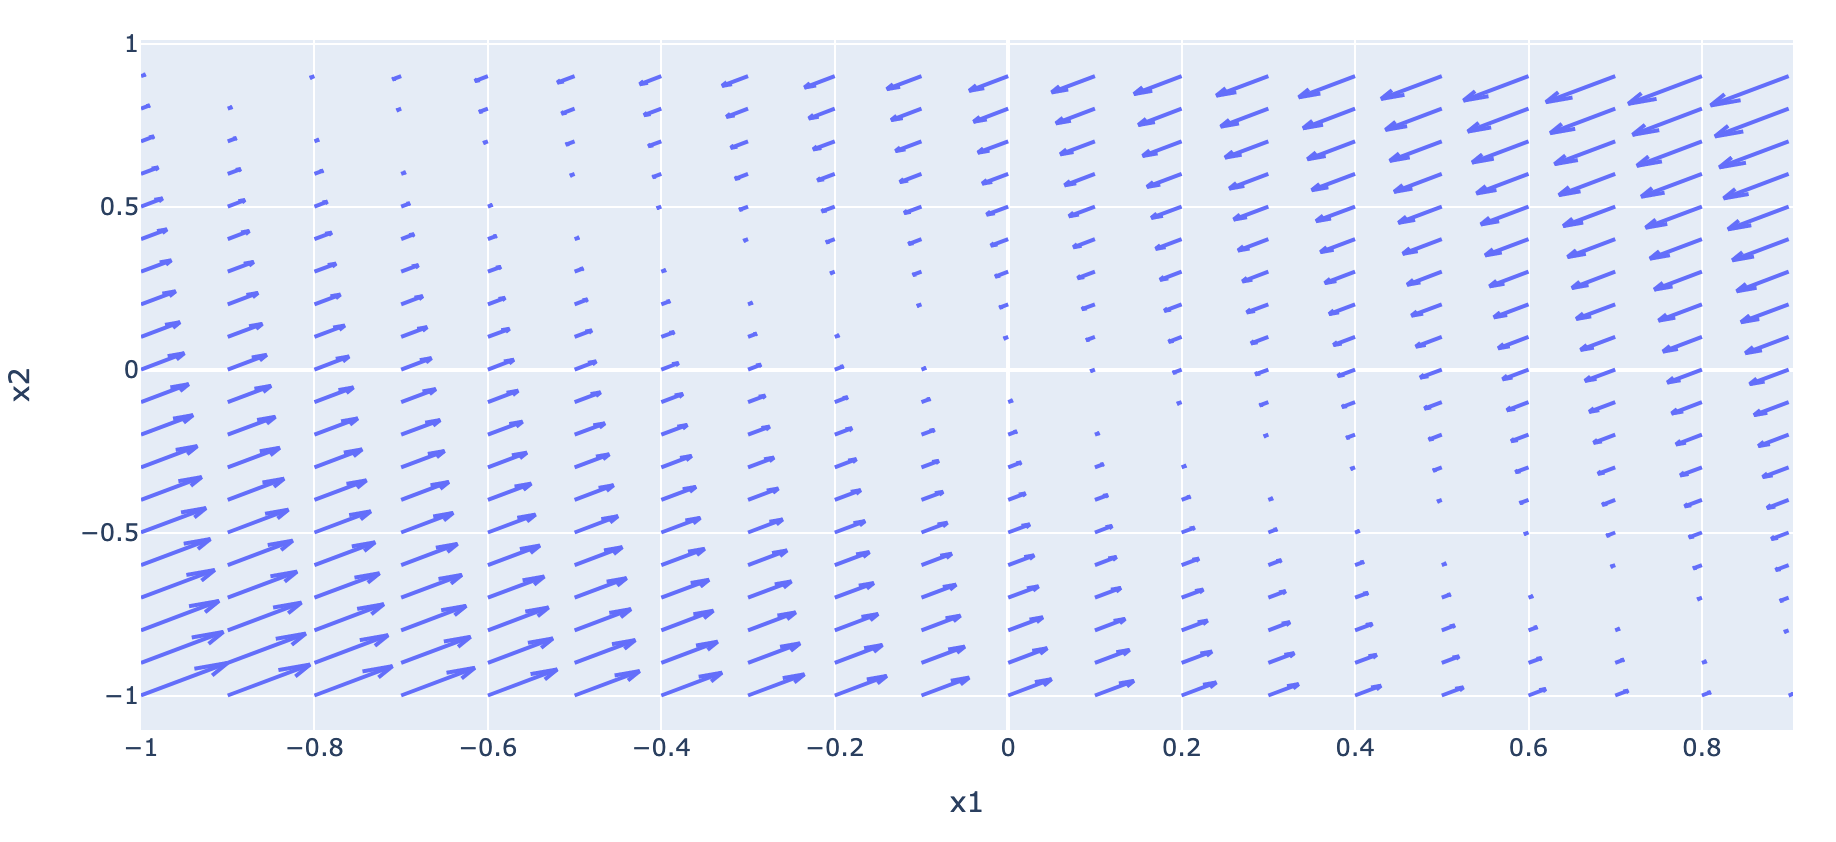
\includegraphics[width=1\textwidth]{Figures/x1x2.png}
    \caption{Projection of $\mathbf{f}(x)=\mathbf{Ax}$ onto a plane defined by $x_{3}=0$.}
\end{figure} 
\begin{figure}[h]
    \centering
    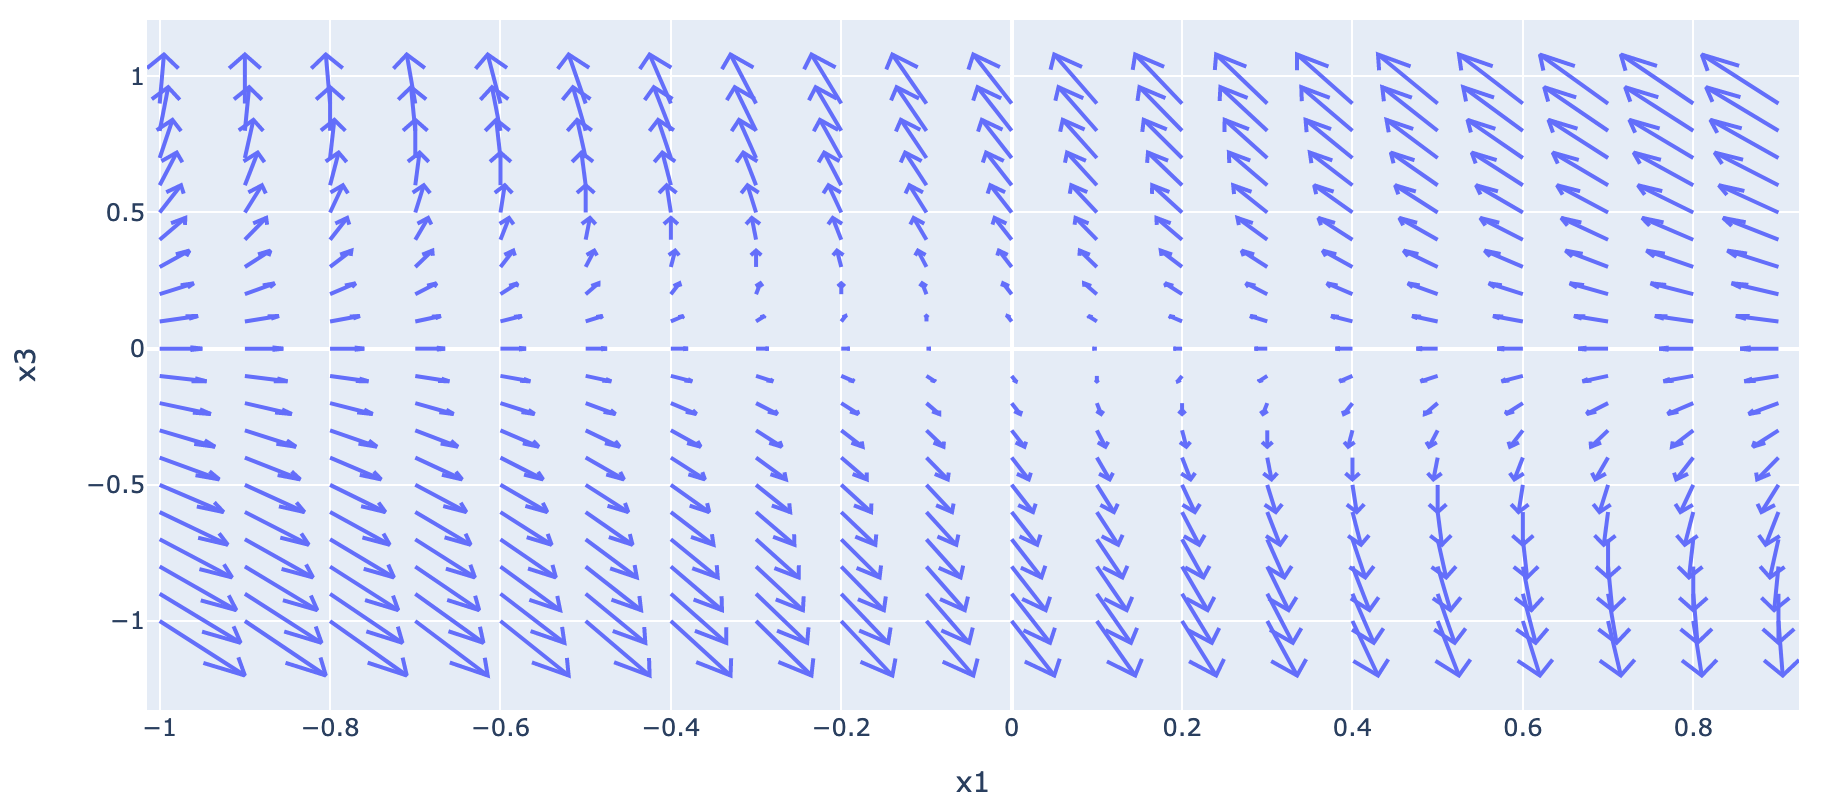
\includegraphics[width=1\textwidth]{Figures/x1x3.png}
    \caption{Projection of $\mathbf{f}(x)=\mathbf{Ax}$ onto a plane defined by $x_{2}=0$.}
\end{figure} 
\begin{figure}[h]
    \centering
    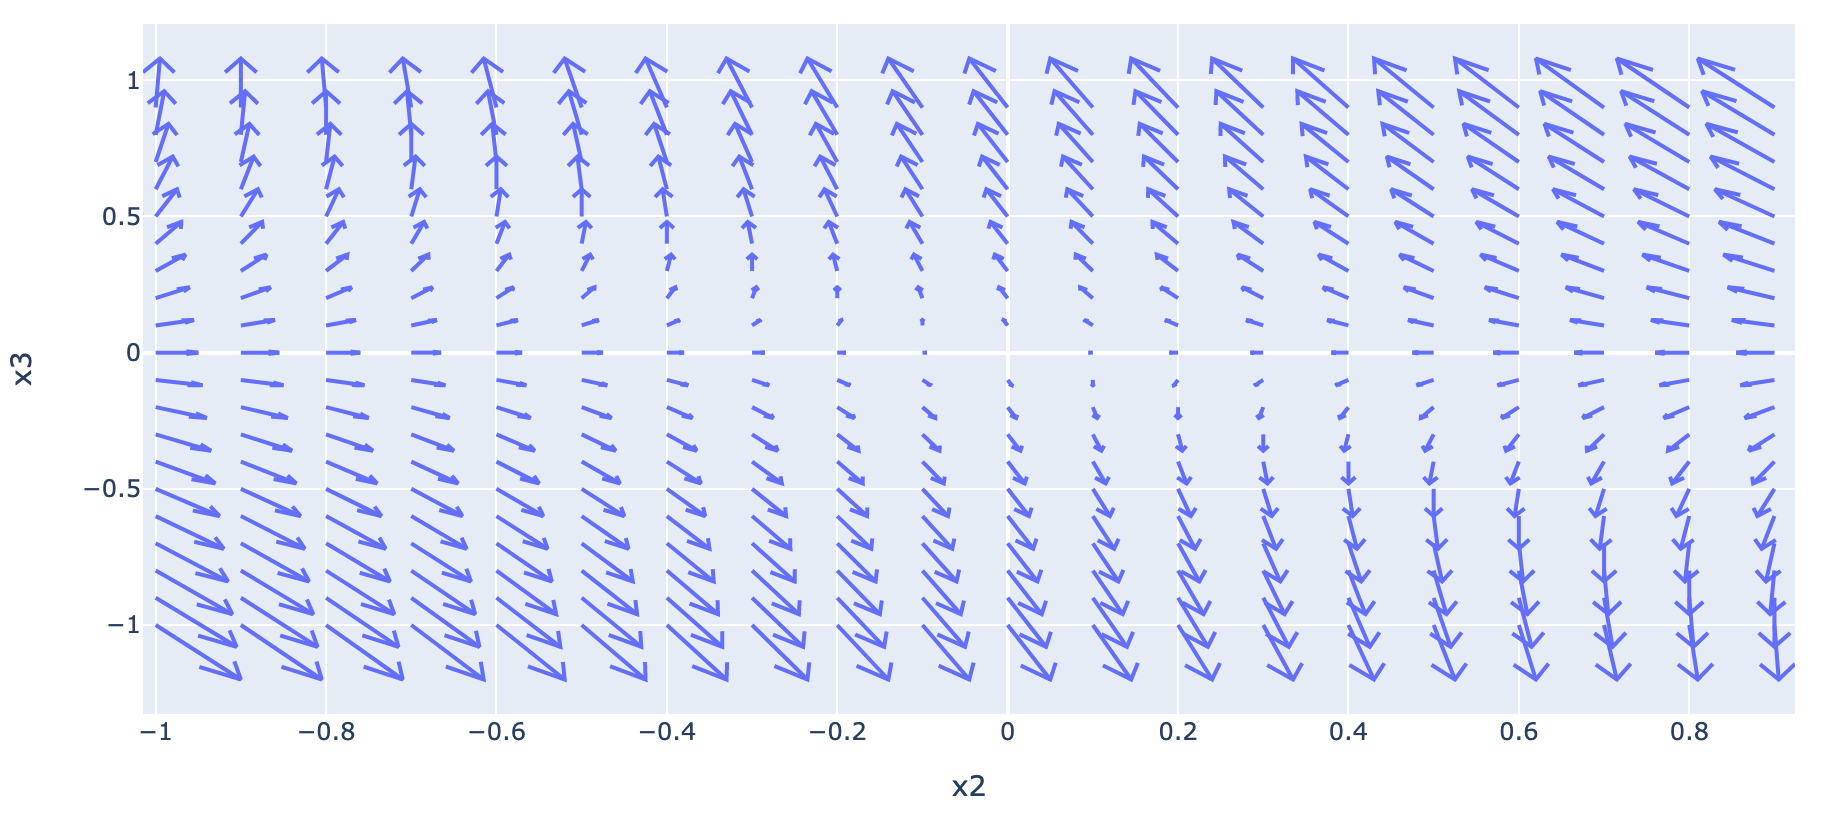
\includegraphics[width=1\textwidth]{Figures/x2x3.png}
    \caption{Projection of $\mathbf{f}(\mathbf{x})=\mathbf{Ax}$ onto a plane defined by $x_{1}=0$.}
\end{figure} 
The dynamics observed in Figure 5 can be explained using the fact that the eigenvalue associated with eigenvector $\mathbf{v}_{1}$ is zero.
Therefore, we see an invariant manifold along the direction of this eigenvector, with particles attracted towards it. As for Figures 6 and 7, there 
is a saddle point at $(0, 0)$, for there is one stable and one unstable direction.
\item[1.4] Now we want to project the vector field of the dynamics onto the subspace defined by the basis
\[
\mathbf{e}_{1}=\frac{1}{\sqrt{2}}\begin{pmatrix}1\\ -1\\ 0\end{pmatrix}, \quad \mathbf{e}_{2}=\begin{pmatrix}0\\ 0\\ 1\end{pmatrix}
\] 
Recall the formula for projecting vector $\mathbf{x}$ onto a line spanned by vector $\mathbf{u}$
\[
    \text{proj}_{\mathbf{u}}(\mathbf{x}) = \frac{\mathbf{u} \cdot \mathbf{x}}{\|\mathbf{u}\|^{2}}\mathbf{u}
\]
Therefore, to project vector $\mathbf{x}$ onto a subspace V spanned by $\mathbf{e}_{1}$ and $\mathbf{e}_{2}$, we need to do the following
\[
    \text{proj}_{V}(\mathbf{x}) = \frac{\mathbf{e}_{1} \cdot \mathbf{x}}{\|\mathbf{e}_{1}\|^{2}}\mathbf{e}_{1} + \frac{\mathbf{e}_{2} \cdot \mathbf{x}}{\|\mathbf{e}_{2}\|^{2}}\mathbf{e}_{2}
\]
And since $\mathbf{e}_{1}$ and $\mathbf{e}_{2}$ form the basis, we know they are unit vectors, and hence we are left with
\[
    \text{proj}_{V}(\mathbf{x}) = \left(\mathbf{e}_{1} \cdot \mathbf{x}\right)\mathbf{e}_{1} + \left(\mathbf{e}_{2} \cdot \mathbf{x}\right)\mathbf{e}_{2}
\]
The eigenvectors $\mathbf{v}_{1}$ and $\mathbf{v}_{2}$ are mapped onto themselves by this projection, and the eigenvector $\mathbf{v}_{3}$ is mapped to $\mathbf{0}$, and hence we 
see an unstable manifold.
\item[1.5] Now we want to compute the stationary solution for $(t \rightarrow \infty)$ with a constant input $\mathbf{s}=\begin{pmatrix}1\\ 2\\ 0\end{pmatrix}$ and the initial condition $\mathbf{x}_{0}=\begin{pmatrix}0\\ 0\\ 0\end{pmatrix}$.
To find the solution, we will use the undetermined coefficients methods to solve this system of inhomogeneous DEQs. Recall that our general solution to the homogeneous system was
\[
    \mathbf{x}(t)=c_{1}\mathbf{v}_{1}e^{\lambda_{1}t} + c_{2}\mathbf{v}_{2}e^{\lambda_{2}t} + c_{3}\mathbf{v}_{3}e^{\lambda_{3}t}
\]
We need to find a particular solution $\mathbf{x}_{p}(t)$, so let
\[
\mathbf{x}_{p}(t)=\begin{pmatrix}x_{1}t + b_{1}\\ x_{2}t + b_{2}\\ 0\end{pmatrix}, \qquad \text{(since our input is constant)}
\]
And now we plug this into our orginal system to find $x_{1}$, $x_{2}$, and $x_{3}$
\begin{align*}
    \begin{pmatrix}x_{1}\\ x_{2}\\ 0\end{pmatrix} &= \mathbf{A}\begin{pmatrix}x_{1}t + b_{1}\\ x_{2}t + b_{2}\\ 0\end{pmatrix} + \mathbf{s}\\
    \implies \begin{pmatrix}x_{1}\\ x_{2}\\ 0\end{pmatrix} &= \begin{pmatrix}-0.5 & -0.5 & 0\\ -0.5 & -0.5 & 0\\0 & 0 & 2\end{pmatrix}\begin{pmatrix}x_{1}t + b_{1}\\ x_{2}t + b_{2}\\ 0\end{pmatrix} + \begin{pmatrix}1\\ 2\\ 0\end{pmatrix}\\
    \implies \begin{pmatrix}x_{1}\\ x_{2}\\ 0\end{pmatrix} &= \begin{pmatrix}-0.5(x_{1}t + b_{1})-0.5(x_{2}t + b_{2})+1\\ -0.5(x_{1}t + b_{1})-0.5(x_{2}t + b_{2})+2\\ 0\end{pmatrix}\\
    x_{1} &= -0.5(x_{1}t + b_{1})-0.5(x_{2}t + b_{2})+1\\
    \implies x_{2} &= -0.5(x_{1}t + b_{1})-0.5(x_{2}t + b_{2})+2\\
    0 &= 0
\end{align*}
Eventually, we find that our particular solution takes the form
\[
\mathbf{x}_{p}(t) = \begin{pmatrix}-t/2\\ t/2+3\\ 0\end{pmatrix}
\]
And the overall general solution for the inhomogeneous DEQ is
\[
    \mathbf{x}(t)=c_{1}\mathbf{v}_{1}e^{\lambda_{1}t} + c_{2}\mathbf{v}_{2}e^{\lambda_{2}t} + c_{3}\mathbf{v}_{3}e^{\lambda_{3}t} + \mathbf{x}_{p}(t)
\]
\end{enumerate}

\newpage
\noindent\textbf{Question 2. Nonlinear Decision Network.}
\begin{enumerate}
    \item[2.1] We are given a system of nonlinear DEQs
\begin{align*}
    \tau \dot{u}_{1}(t) = -u_{1}(t) -c[u_{2}(t) -\Theta]_{+} + s_{1}\\
    \tau \dot{u}_{2}(t) = -u_{2}(t) -c[u_{1}(t) -\Theta]_{+} + s_{2}
\end{align*}
where the linear threshold function is defined by $[x]_{+}=\text{max}(0, x)$.\\
This network model can be re-parameterised as follows
\begin{align*}
    \frac{d\tilde{u}_{1}(\tilde{t})}{d\tilde{t}} = -\tilde{u}_{1}(\tilde{t}) -c[\tilde{u}_{2}(\tilde{t})]_{+} + \tilde{s}_{1}\\
    \frac{d\tilde{u}_{2}(\tilde{t})}{d\tilde{t}} = -\tilde{u}_{2}(\tilde{t}) -c[\tilde{u}_{1}(\tilde{t})]_{+} + \tilde{s}_{2}\\
\end{align*}
where we have 
\begin{align*}
    \tilde{u}_{1}(t) &= u_{1}(t) - \Theta\\
    \tilde{u}_{2}(t) &= u_{2}(t) - \Theta\\
    \tilde{s}_{1} &= s_{1} - \Theta\\
    \tilde{s}_{2} &= s_{2} - \Theta\\
    \tilde{t} &= \frac{t}{\tau}
\end{align*}
For notation purposes, we drop the tilde in the above system.
\item[2.2] The reparameterised system can be written in the matrix form as show below
\[
\mathbf{f}(\mathbf{u}) = -\mathbf{u} - c\begin{pmatrix}0 & 1\\ 1 & 0\end{pmatrix} [\mathbf{u}(\tilde{t})]_{+} + \mathbf{s}
\] 
with $\mathbf{u}=\begin{pmatrix}u_{1}\\ u_{2}\end{pmatrix}$ and $\mathbf{s}=\begin{pmatrix}s_{1}\\ s_{2}\end{pmatrix}$. Assuming $c=2$ and $s_{1}=s_{2}=1$, the vector 
field of this dynamics appears in Figure 8.

\begin{figure}[h]
    \centering
    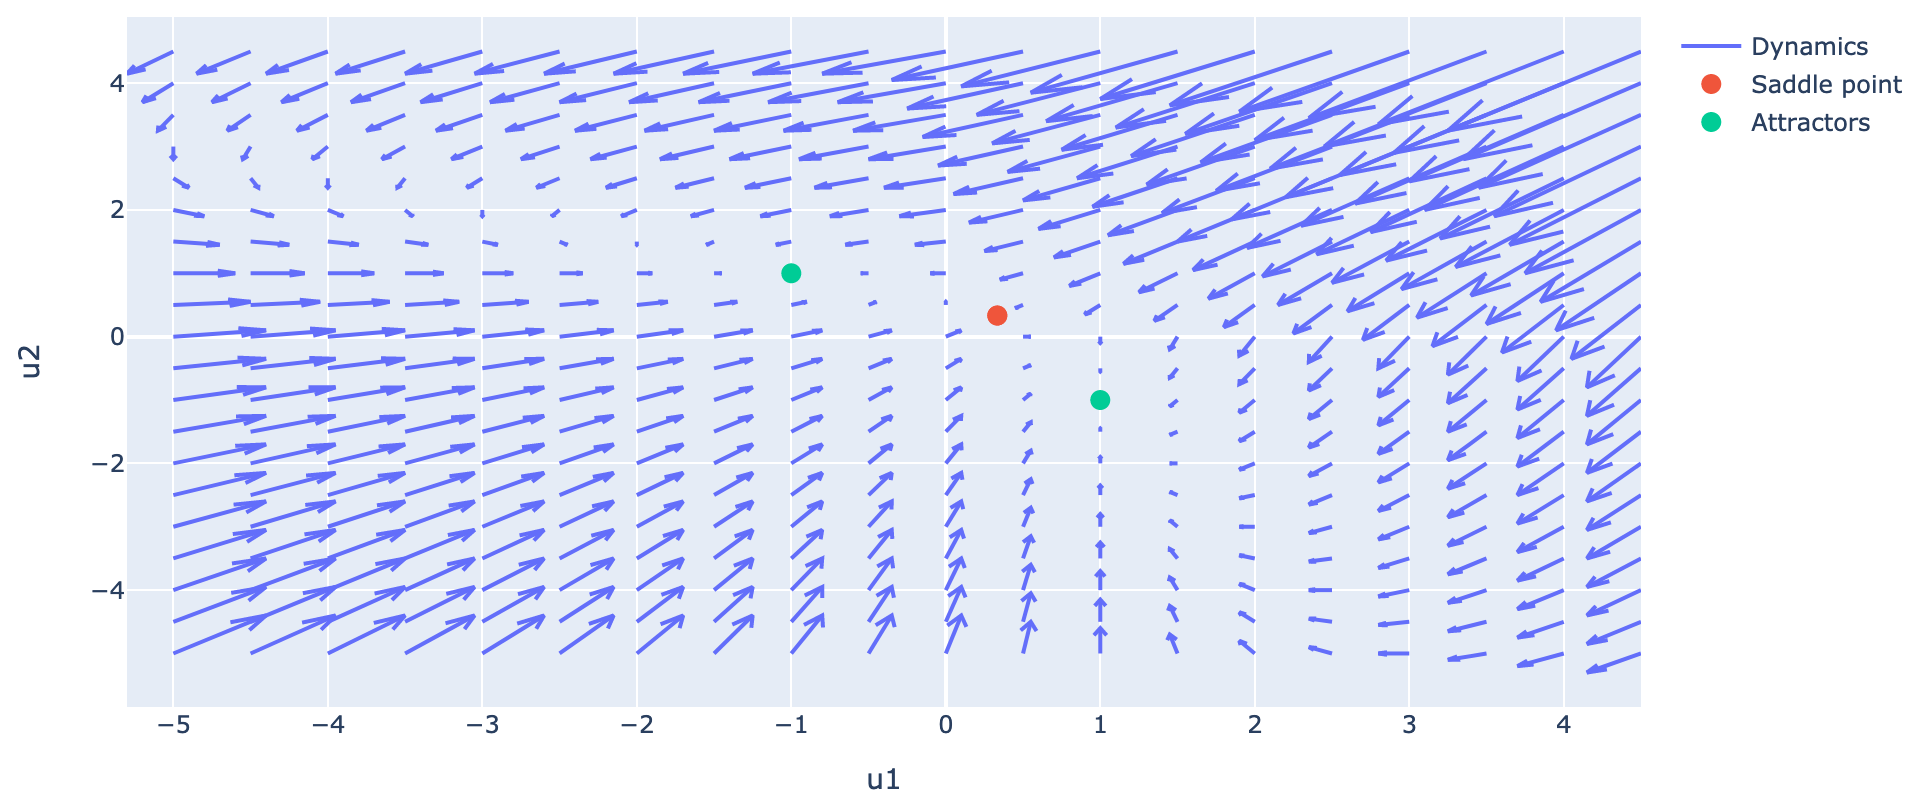
\includegraphics[width=1.1\textwidth]{Figures/u1u2.png}
    \caption{Decision network dynamics with a constant input $s_{1}=s_{2}=1$.}
\end{figure} 

\item[2.3] To compute the fixed points, we evaluate the following equation
\[
    \mathbf{f}(\mathbf{u}) = 0  
\] 
We have
\[
    \systeme*{-u_{1}(t) - 2[u_{2}(t)]_{+} + 1 =0,
    -u_{2}(t) - 2[u_{1}(t)]_{+} + 1=0}
\]
\[
    \implies
    \systeme*{u_{1}(t) + 2[u_{2}(t)]_{+}=1,
    u_{2}(t) + 2[u_{1}(t)]_{+}=1}
\]
\[
    \implies
    \systeme*{u_{1}(t) =1 - 2[u_{2}(t)]_{+},
    u_{2}(t) =1- 2[u_{1}(t)]_{+}}
\]  
Now, we need to consider the four quadrants. For $u_{1}, u_{2} > 0$, we have
\[
    \systeme*{u_{1}(t) = 1-2u_{2}(t), u_{2}(t) = 1-2u_{1}(t)}\\
    \implies \systeme*{u_{1}(t)=\frac{1}{3}, u_{2}(t)=\frac{1}{3}}
\]
Similarly, for $u_{1}>0, u_{2}<0$
\[
    \systeme*{u_{1}(t) = 1, u_{2}(t) = -1}\\
\]
For $u_{1}<0, u_{2}>0$
\[
    \systeme*{u_{1}(t) = -1, u_{2}(t) = 1}\\
\]
For $u_{1}<0, u_{2}<0$ we get a contradiction, thus in this quadrant there are no fixed points.
\item[2.4] To compute the dynamics matrix $\mathbf{A}$, we need to solve for
\[
    0=\mathbf{A}\mathbf{u} + \mathbf{s}  
\] 
Which we have already done in 2.3. As such, we have
\[
\mathbf{A}_{u_{1}>0, u_{2}>0} = \begin{pmatrix} -1 & -2\\ -2 & -1\end{pmatrix}, \quad \mathbf{A}_{u_{1}<0, u_{2}>0} = \begin{pmatrix} -1 & -2\\ 0 & -1\end{pmatrix}, \quad \mathbf{A}_{u_{1}<0, u_{2}<0} = \begin{pmatrix} -1 & 0\\ -2 & -1\end{pmatrix}
\]
We have already showed how to eigendecompose a matrix in 1.1. Thus, following the same procedure, the eigenvalues for $\mathbf{A}_{u_{1}>0, u_{2}>0}$ are $\lambda_{1}=-3$ and $\lambda_{2}=1$, which describes a stable dynamics towards the fixed point (attractor).
For $\mathbf{A}_{u_{1}<0, u_{2}>0}$, there is a single eigenvalue $\lambda=-1$ with algebraic multiplicity 2, which also yeilds an attractor.
Finally, for $\mathbf{A}_{u_{1}<0, u_{2}<0}$ we also have $\lambda=-1$ with algebraic multiplicity 2.
\item[2.5] For the two different inputs, the stationary solutions $\mathbf{u}(\infty)$ for the below initial conditions 
\begin{itemize}
 \item $\mathbf{u}(0) = \mathbf{0}$
\item $\mathbf{u}(0) = \begin{pmatrix}1\\ -1\end{pmatrix}$
\item $\mathbf{u}(0) = \begin{pmatrix}-1\\ 1\end{pmatrix}$
\end{itemize}
were computed numerically using the Forward Euler method approximation. The simulation results appear in Figures 9 and 10.
\begin{figure}[h]
    \centering
    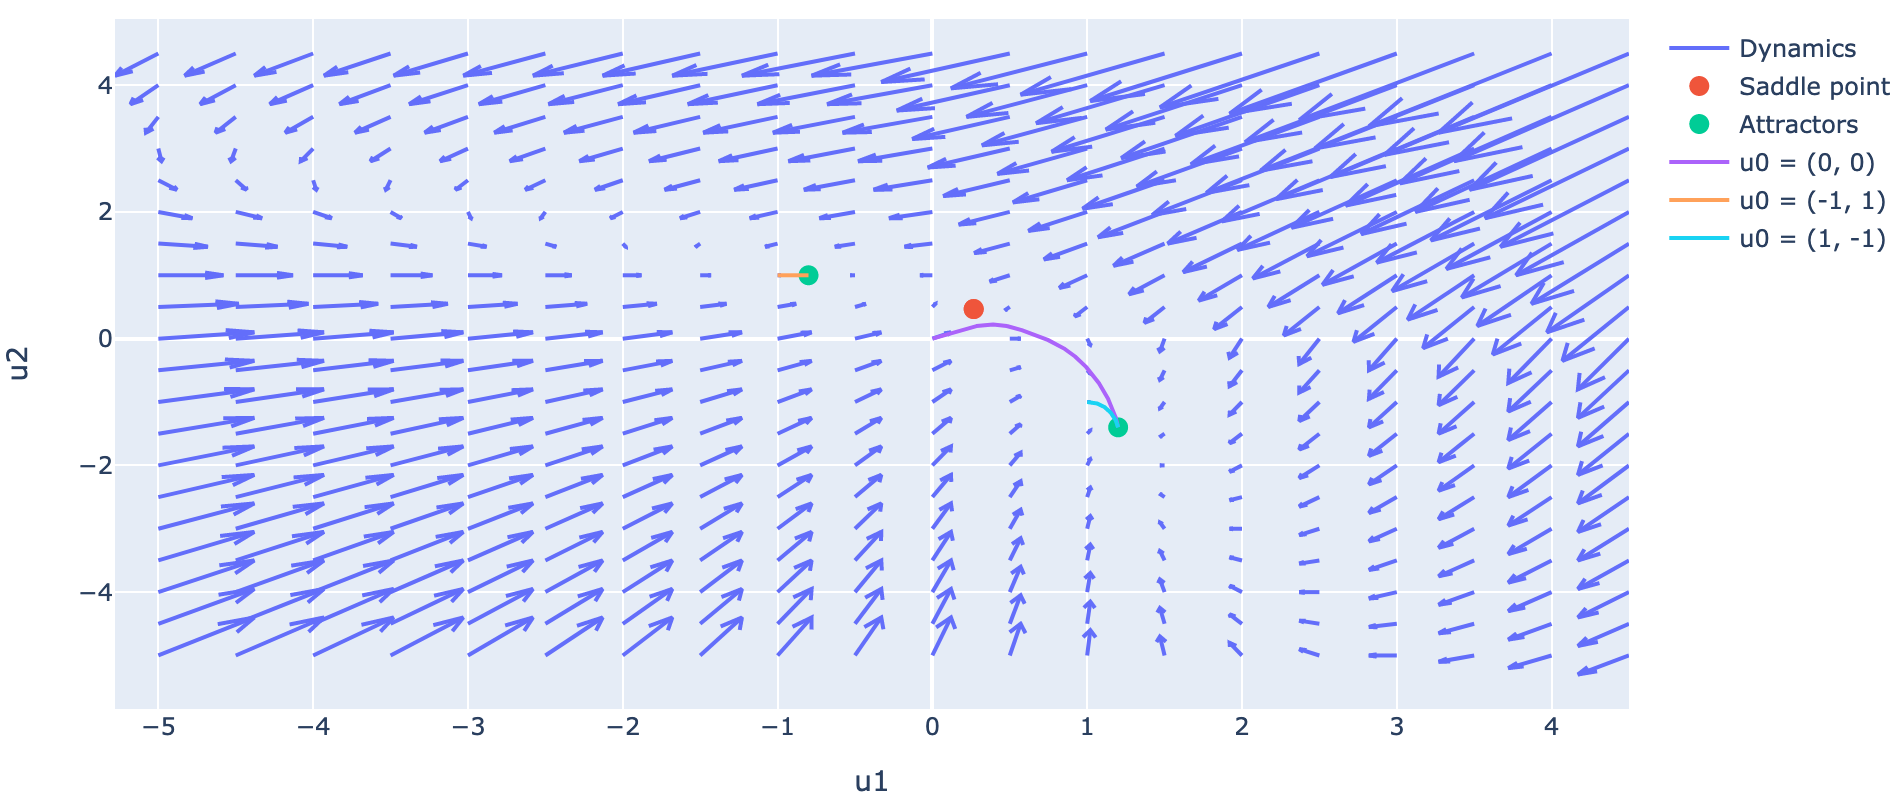
\includegraphics[width=1.1\textwidth]{Figures/121.png}
    \caption{Stationary solutions with the constant input $s_{1}=1.2$, $s_{2}=1$.}
\end{figure} 
\begin{figure}[h]
    \centering
    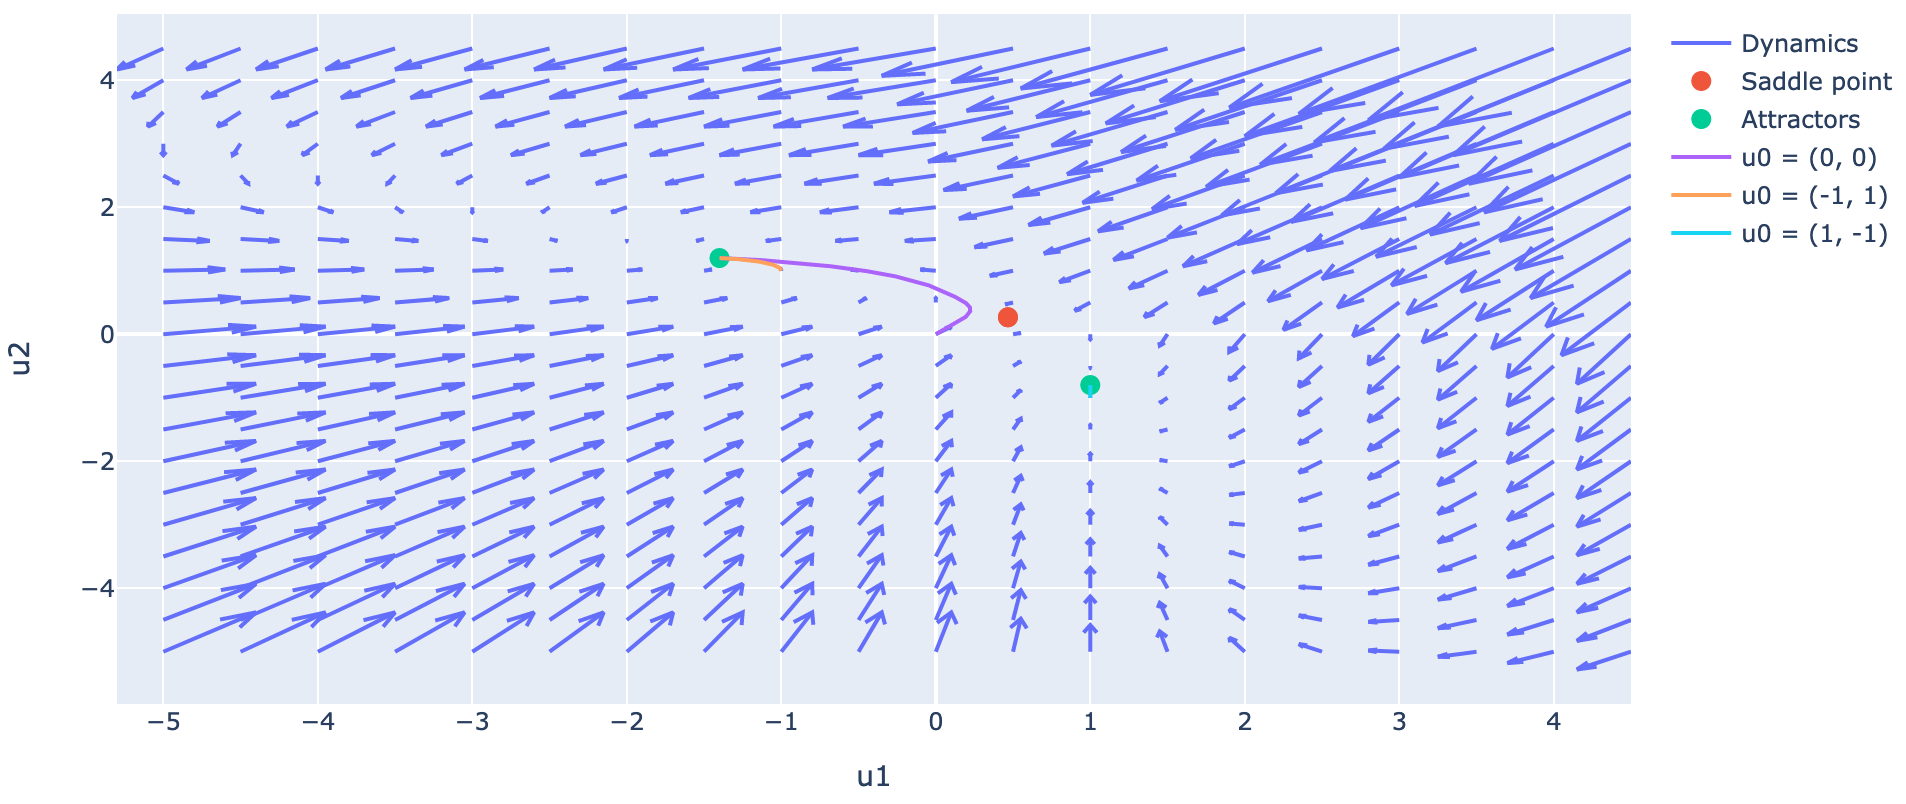
\includegraphics[width=1.1\textwidth]{Figures/112.png}
    \caption{Stationary solutions with the constant input $s_{1}=1$, $s_{2}=1.2$.}
\end{figure} 
As clearly visible from the figures, depending on the input the same initial conditions converge to different attractors. This means that the two neurons 
are able to discriminate between the two input signals by the means of different fixed firing rates.
\item[2.6] For $s_{1}=s_{2}=1$ and $c=-2$ the dynamics and the stationary solutions like like shown in Figure 11. There are 
no fixed points in this system, and hence the solutions do not converge.
\begin{figure}[h]
    \centering
    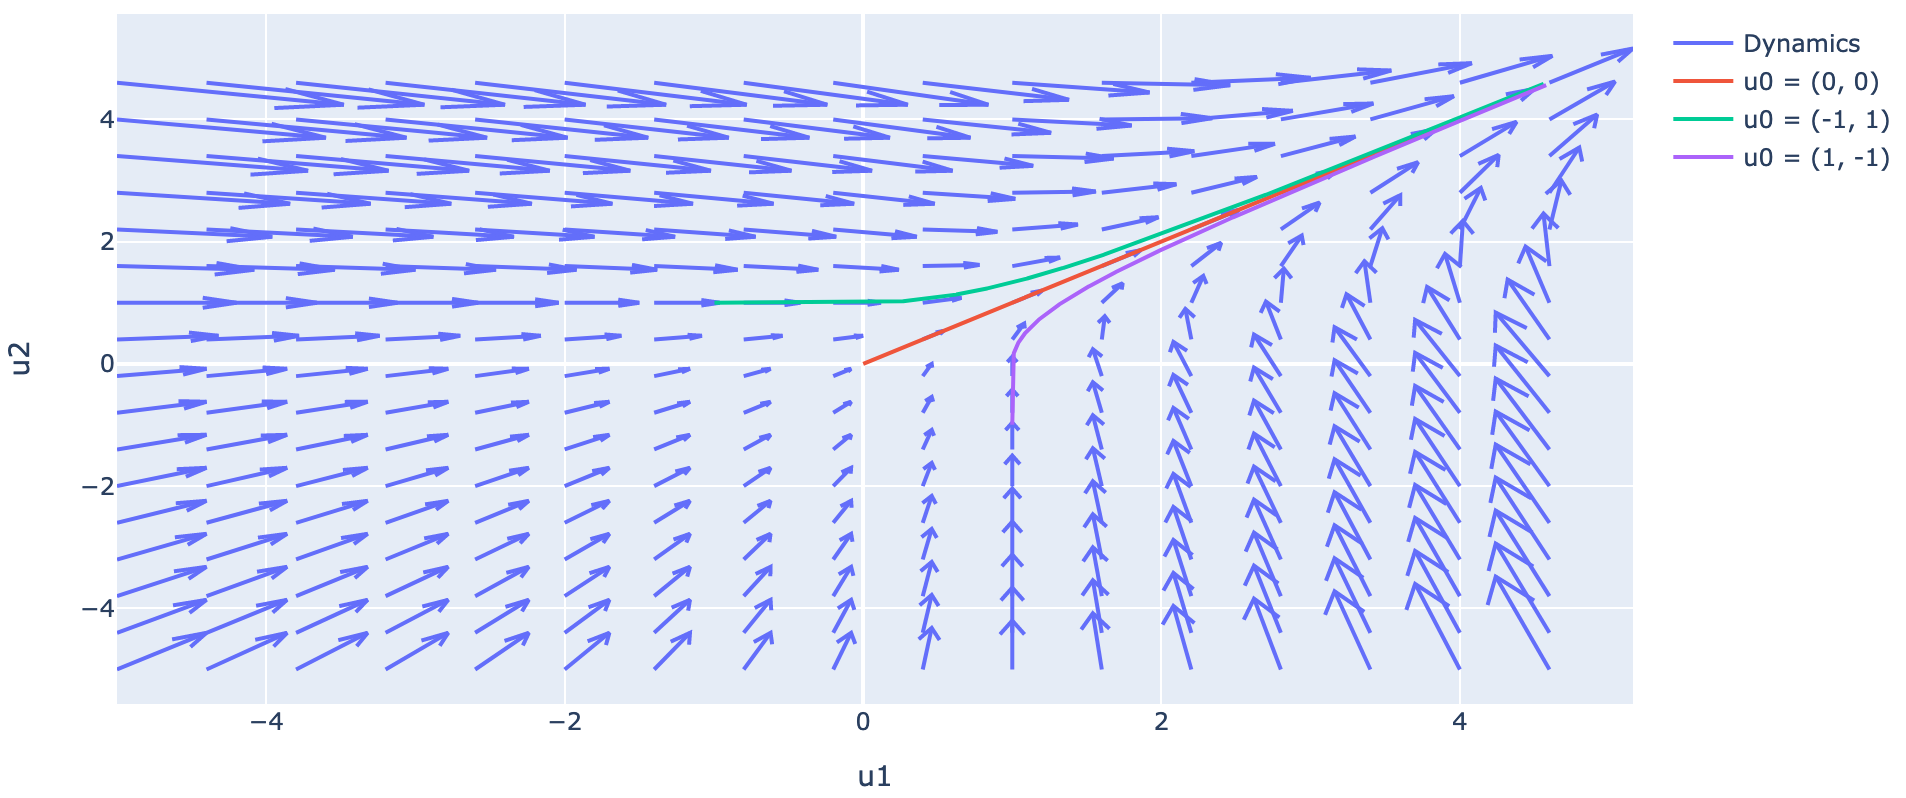
\includegraphics[width=1.1\textwidth]{Figures/c-2.png}
    \caption{Stationary solutions with the constant input $s_{1}=1$, $s_{2}=1.2$ and $c=-2$.}
\end{figure}  
\item[2.7] We now replace the ReLU nonlinearity in our original system with the following step funciton 
\[
    1(x)=\begin{cases}
        1, & (x>0)\\
        0, & (x\leq 0)
    \end{cases}  
\] 
The vector field now changes to what can be seen in Figure 12 along with the stationary solutions specified by the initial conditions in 2.5 and inputs in 2.6.
All the solutions converge towards the attractor at $(3, 3)$, which is obvious from our fixed point computations in 2.3. As opposed to ReLU, our new
nonlinearity introduces an upper bound on convergence. 
\begin{figure}[h]
    \centering
    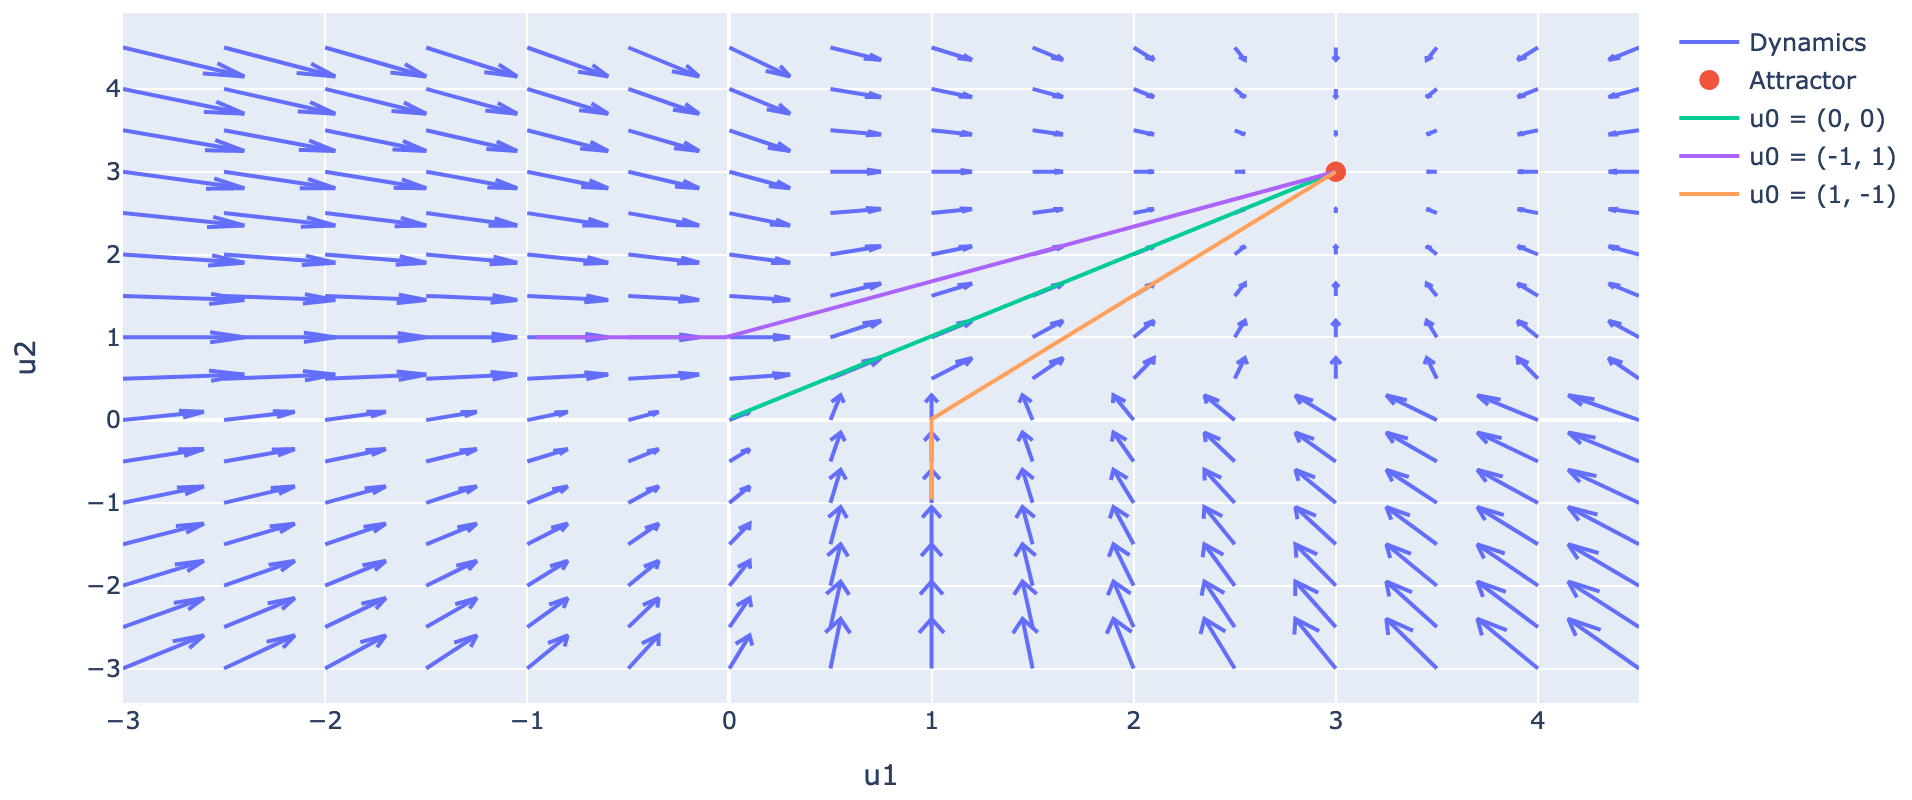
\includegraphics[width=1.1\textwidth]{Figures/one.png}
    \caption{Stationary solutions with the constant input $s_{1}=1$, $s_{2}=1$ and $c=-2$ with the nonlinearity changed to $1(x)$.}
\end{figure}  
\end{enumerate}
\end{document}
